\problemname{Sortera spellistan}
Du har en spellista med $N$ låtar med olika längder som ligger i en given ordning. Du vill sortera listan så att de kortaste
låtarna kommer först och de längsta låtarna kommer sist.

Vad är det minsta antalet platsbyten du behöver göra för att få listan sorterad?
Vid ett platsbyte väljer du två intilliggande låtar och byter plats på dem.

\begin{figure}[ht!]
\centering
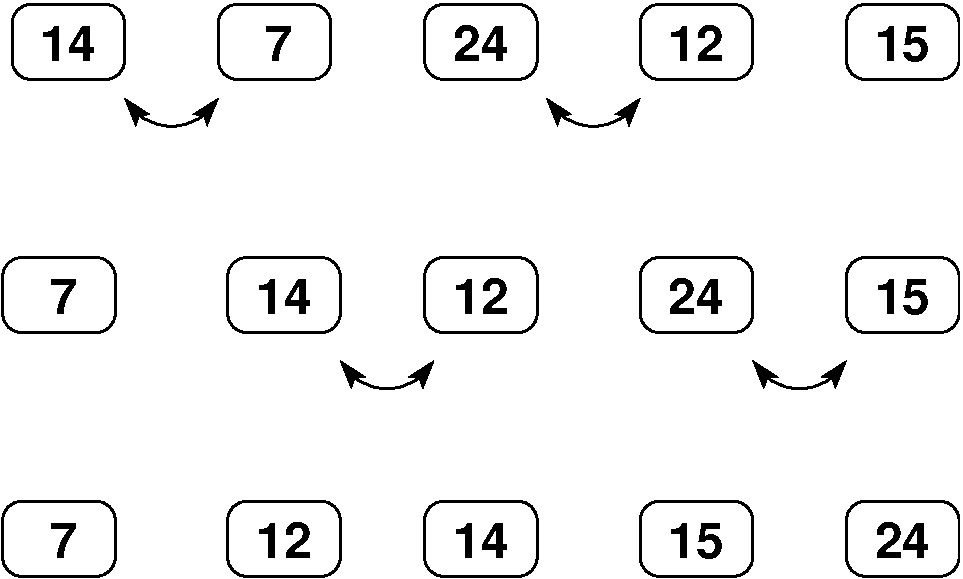
\includegraphics[width=5cm]{sorterafig.pdf}
\caption{Översta raden visar låtarnas startordning i första exemplet. Pilarna visar platsbytena som behöver göras för att göra spellistan sorterad (understa raden)}
\end{figure}

\section*{Indata}
På första raden av indatan står ett heltal $N$, ($1 \leq N \leq 1000$), antalet låtar.

Därefter följer $N$ rader. Varje rad innehåller ett heltal $l$ ($1 \leq l \leq 1000)$, längden på vardera låt.
Alla låtarna har olika längd.

\section*{Utdata}
Skriv ut ett enda tal: det minsta antalet platsbyten som behöver göras för att sortera spellistan.

\section*{Poängsättning}
Din lösning kommer att testas på en mängd testfallsgrupper.
För att få poäng för en grupp så måste du klara alla testfall i gruppen.

\noindent
\begin{tabular}{| l | l | p{12cm} |}
  \hline
  Grupp & Poängvärde & Gränser \\ \hline
  $1$    & $60$        & $N \leq 100$ \\ \hline 
  $2$    & $40$        & Inga ytterligare begränsingar. \\ \hline 
\end{tabular}